\documentclass[../main.tex]{subfiles}
\graphicspath{{\subfix{../images/}}}
\begin{document}
\section*{Term 2 Week 8}

\begin{enumerate}
    \item 
    \(\int \sqrt{1-x}.\sqrt{x+3}\,dx\)

    \(\int \sqrt{-x^2-2x+3}\,dx\)

    Completing the square:

    \(\int \sqrt{-(x^2+2x)+3}\,dx\)

    \(\int \sqrt{-((x+1)^2-1)+3}\,dx\)

    \(\int \sqrt{4-(x+1)^2}\,dx\)

    \begin{figure}[h]
        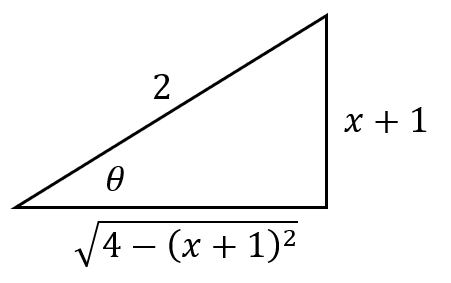
\includegraphics[width=0.25\linewidth]{../images/t2w8q1a.png}
    \end{figure}
    \(\sin{\theta}=\frac{x+1}{2}\\
    x+1=2\sin{\theta}\\
    dx=2\cos{\theta}\,d\theta\)

    Substitute into the integral:\\
    \(\int \sqrt{4-(2\sin{\theta})^2}.2\cos{\theta}\,d\theta\)

    \(\int \sqrt{4-4\sin^2{\theta}}.2\cos{\theta}\,d\theta\)

    \(\int \sqrt{4(1-\sin^2{\theta})}.2\cos{\theta}\,d\theta\)

    \(\int \sqrt{4\cos^2{\theta}}.2\cos{\theta}\,d\theta\)

    \(\int 2\cos{\theta}.2\cos{\theta}\,d\theta\)

    \(4\int \cos^2{\theta}\,d\theta\)

    Using cosine double angle rule, \(\cos{2\theta}=2\cos^2{\theta}-1\), we know \(\cos^2{\theta}=\frac{1}{2}(\cos{2\theta}+1)\)

    \(2\int (\cos{2\theta}+1)\,d\theta=2(\frac{\sin{2\theta}}{2}+\theta)+c=\sin{2\theta}+2\theta+c\)

    Use the sine double angle rule:
    \(2\sin{\theta}\cos{\theta}+2\theta+c\)

    Use the triangle to rewrite in terms of \(x\):
    \(\sin{\theta}=\frac{x+1}{2}, \cos{\theta}=\frac{\sqrt{4-(x+1)^2}}{2}, \theta=\sin^{-1}{\frac{x+1}{2}}\)

    \(\int \sqrt{1-x}.\sqrt{x+3}\,dx=2\frac{x+1}{2}\times \frac{\sqrt{4-(x+1)^2}}{2}+2\times \sin^{-1}{(\frac{x+1}{2})}+c\)

    \(=\frac{(x+1)\sqrt{4-(x+1)^2}}{2}+2\sin^{-1}{(\frac{x+1}{2})}+c\)
    
    \item 
    $
    \sin{x}\cos{y}=\frac{1}{4}\\
    \sin{y}\cos{x}=\frac{3}{4}
    $

    Subtract the equations and use the compound angles formula for sine:\\
    $
    \sin{y}\cos{x}-\sin{x}\cos{y}=\frac{1}{2}\\
    \sin{(y-x)}=\frac{1}{2}\\
    $
    We can solve this using the sine general formula:\\
    Remembering \(\sin^{-1}{(\frac{1}{2})}=\frac{\pi}{6}\)

    \(y-x=n\pi + (-1)^n\times \frac{\pi}{6}\\
    n=0 \Rightarrow : y-x = \frac{\pi}{6}\\
    n=1 \Rightarrow : y-x = \frac{5\pi}{6}\\
    n=-1 \Rightarrow : y-x = \frac{-7\pi}{6}\\
    n=-2 \Rightarrow : y-x = \frac{-11\pi}{6}\\
    \)
    
    Add the equations and use the compound angles formula for sine again:\\
    \(\sin{y}\cos{x}+\sin{x}\cos{y}=1\\
    \sin{(x+y)}=1\)

    We know that \(\sin^{-1}{(1)}=\frac{\pi}{2}\)

    Therefore, \(x+y=\frac{\pi}{2}\)

    Combining the two:

    \((x+y)+(y-x)=2y\)

    Here we find the first solutions either side of the origin. We know that these will repeat every \(2\pi\) so will use these as our principal solutions.

    $
    \!
    \begin{aligned}[t]
        2y
        &=\frac{\pi}{6}+\frac{\pi}{2}=\frac{2\pi}{3}\\
        &=\frac{5\pi}{6}+\frac{\pi}{2}=\frac{4\pi}{3}\\
        &=\frac{-7\pi}{6}+\frac{\pi}{2}=\frac{-2\pi}{3}\\
        &=\frac{-11\pi}{6}+\frac{\pi}{2}=\frac{-4\pi}{3}\\
        y &= \Bigl\{\frac{\pi}{3},\frac{2\pi}{3},-\frac{\pi}{3},-\frac{2\pi}{3}\Bigr\}
    \end{aligned}
    $

    Solving for \(x\):\\
    \(x=\frac{\pi}{2}-y\)

    $
    \!
    \begin{aligned}[t]
        x
        &=\frac{\pi}{2}-\frac{\pi}{3}=\frac{\pi}{6}\\
        &=\frac{\pi}{2}-\frac{2\pi}{3}=-\frac{\pi}{6}\\
        &=\frac{\pi}{2}--\frac{\pi}{3}=\frac{5\pi}{6}\\
        &=\frac{\pi}{2}--\frac{2\pi}{3}=\frac{7\pi}{6}\\
    \end{aligned}
    $

    So our first principal solutions are: \((\frac{\pi}{6}, \frac{\pi}{3}), (\frac{-\pi}{6}, \frac{2\pi}{3}), (\frac{5\pi}{6}, -\frac{\pi}{3}), (\frac{7\pi}{6}, -\frac{2\pi}{3})\)
    
    Since we know the values of each will repeat every \(2\pi\), we can generalise:

    $
    \!
    \begin{aligned}[t]
        (x,y)
        &=(\frac{\pi}{6}\pm 2\pi a, \frac{\pi}{3}\pm 2\pi b)\\
        &=(-\frac{\pi}{6}\pm 2\pi a, \frac{2\pi}{3}\pm 2\pi b)\\
        &=(\frac{5\pi}{6}\pm 2\pi a, -\frac{\pi}{3}\pm 2\pi b)\\
        &=(\frac{7\pi}{6}\pm 2\pi a, -\frac{2\pi}{3}\pm 2\pi b)
    \end{aligned}
    $

\end{enumerate}

\end{document}

